\chapter{Retropropagación en capas convolucionales} \label{backprop_conv_apendice}

\begin{figure}[H]
	\centering
	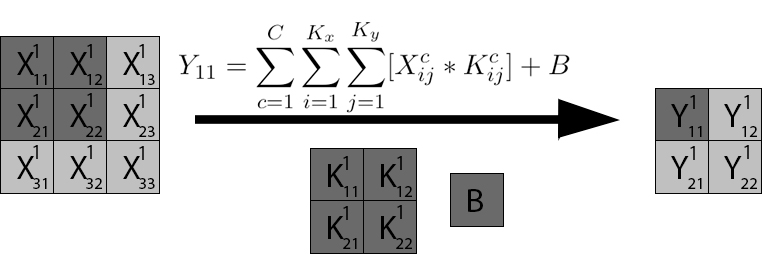
\includegraphics[width=0.8\linewidth]{imagenes/conv_ejemplo_backprop_1.jpg} 
	\caption{Ejemplo de propagación hacia delante en una capa convolucional}
	\label{fig:ejemplo_forward_prop_convolucional_apendice}
\end{figure}

La figura \ref{fig:ejemplo_forward_prop_convolucional_apendice} ilustra el ejemplo de propagación hacia delante que se utilizará en esta sección. En dicha figura, \textit{C} representa el número de canales de profundidad del volumen de entrada \textit{X}, mientras que ${K_x}$ y ${K_y}$ se refieren al número de filas y columnas del kernel \textit{K} utilizado, respectivamente. \\
Siguiendo la notación empleada en secciones anteriores, se denotará por $A^c_{ij}$ al valor de $X^c_{ij}$ antes de aplicar la función de activación correspondiente, y por $Z^c_{ij}$, al valor resultante después de aplicar dicha función.

\section{Sumatoria de gradientes}

\begin{gather}
	\frac{\partial E}{\partial K^c_{11}} = \sum_{i=1}^{I}\sum_{j=1}^{J}  [\frac{\partial E}{\partial Y^c_{ij}} * \frac{\partial Y^c_{ij}}{\partial K^c_{11}}] \\
	\frac{\partial E}{\partial X^c_{11}} = \sum_{i=1}^{I}\sum_{j=1}^{J}  [\frac{\partial E}{\partial Y^c_{ij}} * \frac{\partial Y^c_{ij}}{\partial Z^c_{11}} * \frac{\partial Z^c_{ij}}{\partial A^c_{11}}] 
\end{gather}

Para calcular el gradiente de la función de error con respecto a cada peso ${K_{xy}}$ o entrada ${X_{xy}}$, se debe realizar una sumatoria del gradiente correspondiente sobre cada valor de salida producido por la convolución. En el caso de los pesos asociados a un canal de profundidad $c \in C$, cada peso ${K_{xy}}$ se empleó en el cálculo de cada valor $Y^c_{ij}$. Por otro lado, los valores de la entrada ${X_{xy}}$ contribuyen al cálculo de varios valores de salida $\{Y_1, Y_2\} \in Y$. Este proceso fue detallado anteriormente en la sección \ref{intro_CNN}.

\subsection{Gradiente de $Y^c_{11}$}

\begin{gather}
	Y^c_{11} = Z^c_{11} * K^c_{11} + Z^c_{12} * K^c_{12} + Z^c_{21} * K^c_{21} + Z^c_{22} * K^c_{22} \label{grad_y11_k_11_apendice} \\
	\frac{\partial Y^c_{11}}{\partial K^c_{xy}} = \frac{\partial (Z^c_{11} * K^c_{11} + Z^c_{12} * K^c_{12} + Z^c_{21} * K^c_{21} + Z^c_{22} * K^c_{22})}{\partial K^c_{xy}} \label{grad_y11_k_12_apendice} \\
	\frac{\partial Y^c_{11}}{\partial K^c_{11}} = Z^c_{11}, \hspace{10mm} \frac{\partial Y^c_{11}}{\partial K^c_{12}} = Z^c_{12} \label{grad_y11_k_21_apendice}\\
	\frac{\partial Y^c_{11}}{\partial K^c_{21}} = Z^c_{21}, \hspace{10mm} \frac{\partial Y^c_{11}}{\partial K^c_{22}} = Z^c_{22} \label{grad_y11_k_22_apendice}
\end{gather}

\begin{gather}
	\frac{\partial Y^c_{11}}{\partial Z^c_{11}} = K^c_{11}, \hspace{10mm} \frac{\partial Y^c_{11}}{\partial Z^c_{12}} = K^c_{12}, \hspace{10mm} \frac{\partial Y^c_{11}}{\partial Z^c_{13}} = 0 \label{grad_y11_z_1} \\
	\frac{\partial Y^c_{11}}{\partial Z^c_{21}} = K^c_{21}, \hspace{10mm} \frac{\partial Y^c_{11}}{\partial Z^c_{22}} = K^c_{22}, \hspace{10mm} \frac{\partial Y^c_{11}}{\partial Z^c_{23}} = 0 \label{grad_y11_z_2} \\
	\frac{\partial Y^c_{11}}{\partial Z^c_{31}} = 0, \hspace{15mm} \frac{\partial Y^c_{11}}{\partial Z^c_{32}} = 0, \hspace{15mm} \frac{\partial Y^c_{11}}{\partial Z^c_{33}} = 0 \label{grad_y11_z_3}
\end{gather}

La fórmula \ref{grad_y11_k_11_apendice}, presenta una descomposición de $Y^c_{11}$ en términos de $Z$ y $K$. Esto, es esencial para el cálculo del gradiente, tanto con respecto a Z, (como se detalla en las fórmulas \ref{grad_y11_z_1}, \ref{grad_y11_z_2}, \ref{grad_y11_z_3}), como con respecto a K, (como se muestra en las fórmulas \ref{grad_y11_k_12_apendice}, \ref{grad_y11_k_21_apendice}, \ref{grad_y11_k_22_apendice}). Esta descomposición, permite calcular el gradiente de $Y^c_{11}$ con respecto a cada parámetro de la capa convolucional. \\
Cabe destacar que, para calcular el gradiente con respecto a cada valor del volumen de entrada (X), también debe calcularse la derivada de la función de activación asociada a dicha capa. Es decir, $\frac{\partial Z}{\partial A}$. Sin embargo, dado que este proceso ha sido abordado en secciones anteriores, se omitirá en esta ocasión, al igual que el cálculo del gradiente con respecto al sesgo de cada capa. El propósito de esta omisión es evitar cálculos redundantes y concentrar la atención en los aspectos más relevantes e innovadores. No obstante, es importante señalar que todos los cálculos discutidos en esta documentación, y más, están implementados en el código correspondiente, lo que garantiza que este conocimiento se ha aplicado y verificado en la práctica. \\
Además, dado que todo ha sido realizado manualmente por la misma persona, la mayoría de las variables e índices utilizados en la documentación coinciden perfectamente o son muy similares a los empleados en el código. Esto asegura que cualquier lector con conocimientos básicos de programación pueda comprender gran parte de las implementaciones desarrolladas en este proyecto.

\subsection{Gradiente de $Y^c_{12}$}

\begin{figure}[H]
	\centering
	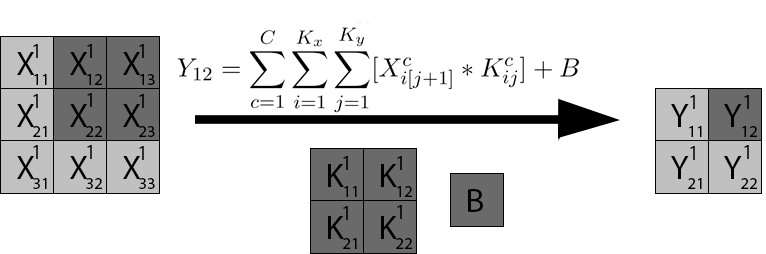
\includegraphics[width=1\linewidth]{imagenes/conv_ejemplo_backprop_2.jpg} 
	\caption{Cálculo de $Y^c_{12}$ mediante propagación hacia delante en una capa convolucional}
	\label{fig:ejemplo_2_forward_prop_convolucional}
\end{figure}

Del mismo modo, se calcula el gradiente de $Y^c_{12}$ con respecto a cada peso, como se muestra en las fórmulas \ref{grad_y12_k_1} y \ref{grad_y12_k_2}.

\begin{gather}
	Y^c_{12} = Z^c_{12} * K^c_{11} + Z^c_{13} * K^c_{12} + Z^c_{22} * K^c_{21} + Z^c_{23} * K^c_{22} \\
	\frac{\partial Y^c_{12}}{\partial K^c_{xy}} = \frac{\partial (Z^c_{11} * K^c_{11} + Z^c_{12} * K^c_{12} + Z^c_{21} * K^c_{21} + Z^c_{22} * K^c_{22})}{\partial K^c_{xy}} \\
	\frac{\partial Y^c_{12}}{\partial K^c_{11}} = Z^c_{12}, \hspace{10mm} \frac{\partial Y^c_{12}}{\partial K^c_{12}} = Z^c_{13} \label{grad_y12_k_1} \\
	\frac{\partial Y^c_{12}}{\partial K^c_{21}} = Z^c_{22}, \hspace{10mm} \frac{\partial Y^c_{12}}{\partial K^c_{22}} = Z^c_{23} \label{grad_y12_k_2}
\end{gather}

Asimismo, se calcula el gradiente de $Y^c_{12}$ con respecto a cada valor de entrada, como se detalla en las fórmulas \ref{grad_y12_z_1}, \ref{grad_y12_z_2} y \ref{grad_y12_z_3}.

\begin{gather}
	\frac{\partial Y^c_{12}}{\partial Z^c_{11}} = 0, \hspace{10mm} \frac{\partial Y^c_{12}}{\partial Z^c_{12}} = K^c_{11}, \hspace{10mm} \frac{\partial Y^c_{12}}{\partial Z^c_{13}} = K^c_{12} \label{grad_y12_z_1} \\
	\frac{\partial Y^c_{12}}{\partial Z^c_{21}} = 0, \hspace{10mm} \frac{\partial Y^c_{12}}{\partial Z^c_{22}} = K^c_{21}, \hspace{10mm} \frac{\partial Y^c_{12}}{\partial Z^c_{23}} = K^c_{22} \label{grad_y12_z_2} \\
	\frac{\partial Y^c_{12}}{\partial Z^c_{31}} = 0, \hspace{10mm} \frac{\partial Y^c_{12}}{\partial Z^c_{32}} = 0, \hspace{15mm} \frac{\partial Y^c_{12}}{\partial Z^c_{33}} = 0 \hspace{5mm} \label{grad_y12_z_3}
\end{gather}

\subsection{Gradiente de $Y^c_{21}$}

\begin{figure}[H]
	\centering
	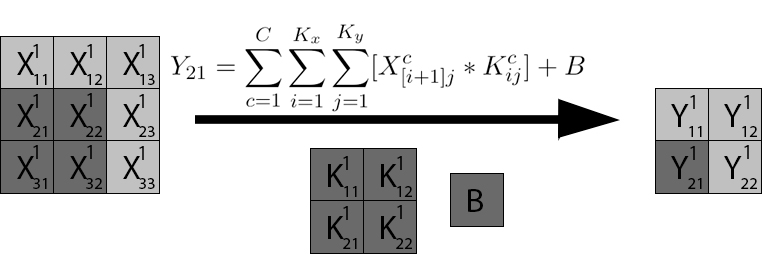
\includegraphics[width=1\linewidth]{imagenes/conv_ejemplo_backprop_3.jpg} 
	\caption{Cálculo de $Y^c_{21}$ mediante propagación hacia delante en una capa convolucional}
	\label{fig:ejemplo_3_forward_prop_convolucional}
\end{figure}

Se calcula el gradiente de $Y^c_{21}$ con respecto a cada peso, tal y como se muestra en las ecuaciones \ref{grad_y21_k_1} y \ref{grad_y21_k_2}.

\begin{gather}
	Y^c_{21} = Z^c_{21} * K^c_{11} + Z^c_{22} * K^c_{12} + Z^c_{31} * K^c_{21} + Z^c_{32} * K^c_{22} \\
	\frac{\partial Y^c_{21}}{\partial K^c_{xy}} = \frac{\partial (Z^c_{21} * K^c_{11} + Z^c_{22} * K^c_{12} + Z^c_{31} * K^c_{21} + Z^c_{32} * K^c_{22})}{\partial K^c_{xy}} \\
	\frac{\partial Y^c_{21}}{\partial K^c_{11}} = Z^c_{21}, \hspace{10mm} \frac{\partial Y^c_{21}}{\partial K^c_{12}} = Z^c_{22} \label{grad_y21_k_1} \\
	\frac{\partial Y^c_{21}}{\partial K^c_{21}} = Z^c_{31}, \hspace{10mm} \frac{\partial Y^c_{21}}{\partial K^c_{22}} = Z^c_{32} \label{grad_y21_k_2}
\end{gather}

Asimismo, se calcula el gradiente de $Y^c_{21}$ con respecto a cada valor de entrada, según se detalla en las ecuaciones \ref{grad_y21_z_1}, \ref{grad_y21_z_2} y \ref{grad_y21_z_3}.

\begin{gather}
	\frac{\partial Y^c_{21}}{\partial Z^c_{11}} = 0, \hspace{16mm} \frac{\partial Y^c_{21}}{\partial Z^c_{12}} = 0, \hspace{13mm} \frac{\partial Y^c_{21}}{\partial Z^c_{13}} = 0 \label{grad_y21_z_1} \\
	\frac{\partial Y^c_{21}}{\partial Z^c_{21}} = K^c_{11}, \hspace{10mm} \frac{\partial Y^c_{21}}{\partial Z^c_{22}} = K^c_{12}, \hspace{10mm} \frac{\partial Y^c_{21}}{\partial Z^c_{23}} = 0 \label{grad_y21_z_2} \\
	\frac{\partial Y^c_{21}}{\partial Z^c_{31}} = K^c_{21}, \hspace{10mm} \frac{\partial Y^c_{21}}{\partial Z^c_{32}} = K^c_{22}, \hspace{10mm} \frac{\partial Y^c_{21}}{\partial Z^c_{33}} = 0 \label{grad_y21_z_3}
\end{gather}


\subsection{Gradiente de $Y^c_{22}$}

\begin{figure}[H]
	\centering
	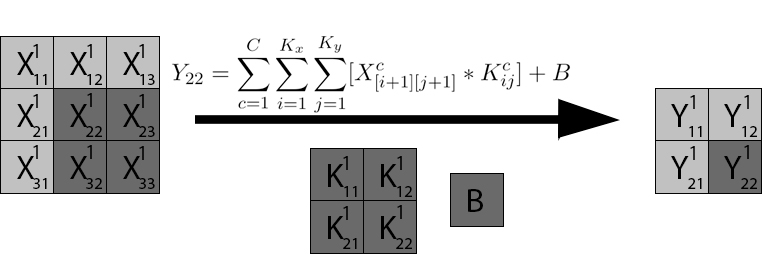
\includegraphics[width=1\linewidth]{imagenes/conv_ejemplo_backprop_4.jpg} 
	\caption{Cálculo de $Y^c_{22}$ mediante propagación hacia delante en una capa convolucional}
	\label{fig:ejemplo_4_forward_prop_convolucional}
\end{figure}

El gradiente de $Y^c_{22}$ se calcula con respecto a cada peso, como se muestra en las fórmulas \ref{grad_y22_k_1} y \ref{grad_y22_k_2}.

\begin{gather}
	Y^c_{22} = Z^c_{22} * K^c_{11} + Z^c_{23} * K^c_{12} + Z^c_{32} * K^c_{21} + Z^c_{33} * K^c_{22} \\
	\frac{\partial Y^c_{22}}{\partial K^c_{xy}} = \frac{\partial (Z^c_{11} * K^c_{11} + Z^c_{12} * K^c_{12} + Z^c_{21} * K^c_{21} + Z^c_{22} * K^c_{22})}{\partial K^c_{xy}} \\
	\frac{\partial Y^c_{22}}{\partial K^c_{11}} = Z^c_{22}, \hspace{10mm} \frac{\partial Y^c_{22}}{\partial K^c_{12}} = Z^c_{23} \label{grad_y22_k_1} \\
	\frac{\partial Y^c_{22}}{\partial K^c_{21}} = Z^c_{32}, \hspace{10mm} \frac{\partial Y^c_{22}}{\partial K^c_{22}} = Z^c_{33} \label{grad_y22_k_2}
\end{gather}

Se calcula el gradiente de $Y^c_{22}$ respecto a cada valor del volumen de entrada, como se muestra en las fórmulas \ref{grad_y22_z_1}, \ref{grad_y22_z_2}, y \ref{grad_y22_z_3}.

\begin{gather}
	\frac{\partial Y^c_{22}}{\partial Z^c_{11}} = 0, \hspace{10mm} \frac{\partial Y^c_{22}}{\partial Z^c_{12}} = 0, \hspace{15mm} \frac{\partial Y^c_{22}}{\partial Z^c_{13}} = 0 \hspace{4mm} \label{grad_y22_z_1} \\
	\frac{\partial Y^c_{22}}{\partial Z^c_{21}} = 0, \hspace{10mm} \frac{\partial Y^c_{22}}{\partial Z^c_{22}} = K^c_{11}, \hspace{10mm} \frac{\partial Y^c_{22}}{\partial Z^c_{23}} = K^c_{12} \label{grad_y22_z_2} \\
	\frac{\partial Y^c_{22}}{\partial Z^c_{31}} = 0, \hspace{10mm} \frac{\partial Y^c_{22}}{\partial Z^c_{32}} = K^c_{21}, \hspace{10mm} \frac{\partial Y^c_{22}}{\partial Z^c_{33}} = K^c_{22} \label{grad_y22_z_3}
\end{gather}

\subsection{Gradiente respecto a pesos como convolución}

Finalmente, se procede al cálculo de la suma total de gradientes con respecto a cada peso de la capa, conforme a las fórmulas \ref{grad_Y_K_1_apendice}, \ref{grad_Y_K_2_apendice}, \ref{grad_Y_K_3_apendice}, y \ref{grad_Y_K_4_apendice}. Se observa un patrón claro en los gradientes resultantes, que refleja la contribución de cada peso en el cálculo del error total.

\begin{gather}
	\frac{\partial E}{\partial K^c_{11}} = \frac{\partial E}{\partial Y^c_{11}} * Z^c_{11} + \frac{\partial E}{\partial Y^c_{12}} * Z^c_{12} + \frac{\partial E}{\partial Y^c_{21}} * Z^c_{21} + \frac{\partial E}{\partial Y^c_{22}} * Z^c_{22} \label{grad_Y_K_1_apendice} \\
	\frac{\partial E}{\partial K^c_{12}} = \frac{\partial E}{\partial Y^c_{11}} * Z^c_{12} + \frac{\partial E}{\partial Y^c_{12}} * Z^c_{13} + \frac{\partial E}{\partial Y^c_{21}} * Z^c_{22} + \frac{\partial E}{\partial Y^c_{22}} * Z^c_{23} \label{grad_Y_K_2_apendice} \\	
	\frac{\partial E}{\partial K^c_{21}} = \frac{\partial E}{\partial Y^c_{11}} * Z^c_{21} + \frac{\partial E}{\partial Y^c_{12}} * Z^c_{22} + \frac{\partial E}{\partial Y^c_{31}} * Z^c_{21} + \frac{\partial E}{\partial Y^c_{22}} * Z^c_{32} \label{grad_Y_K_3_apendice} \\
	\frac{\partial E}{\partial K^c_{22}} = \frac{\partial E}{\partial Y^c_{11}} * Z^c_{22} + \frac{\partial E}{\partial Y^c_{12}} * Z^c_{23} + \frac{\partial E}{\partial Y^c_{31}} * Z^c_{32} + \frac{\partial E}{\partial Y^c_{22}} * Z^c_{33} \label{grad_Y_K_4_apendice}
\end{gather}

Como se observa en los cálculos realizados, estos coinciden con una operación de convolución entre la entrada \textit{X} y el gradiente respecto a la capa de salida \textit{Y}. Este procedimiento se detalla en la Figura \ref{fig:conv_backprop_como_convolucion_X_Y_apendice} \cite{conv_backprop}.

\begin{figure}[H]
	\centering
	\begin{subfigure}{.5\textwidth}
		\hspace{-25mm}
		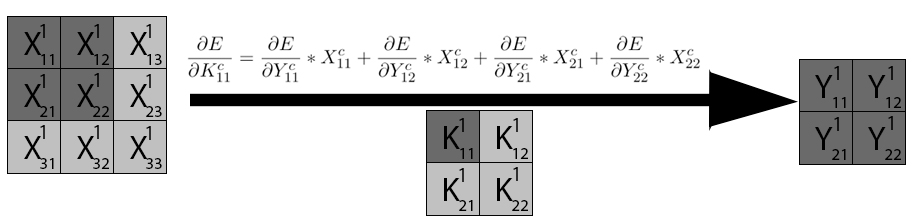
\includegraphics[width=1.4\linewidth]{imagenes/conv_backprop_1.jpg}  
		\caption{Cálculo de $\frac{\partial E}{\partial K^1_{11}}$}
	\end{subfigure}%
	\begin{subfigure}{.5\textwidth}
		\hspace{5mm}
		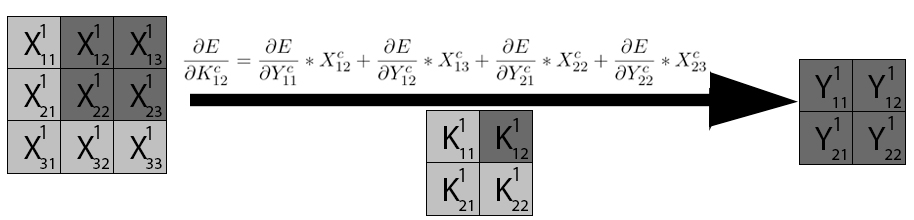
\includegraphics[width=1.4\linewidth]{imagenes/conv_backprop_2.jpg}  
		\caption{Cálculo de $\frac{\partial E}{\partial K^1_{12}}$}
	\end{subfigure}
	\vspace{5mm}
	\begin{subfigure}{.5\textwidth}
		\hspace{-25mm}
		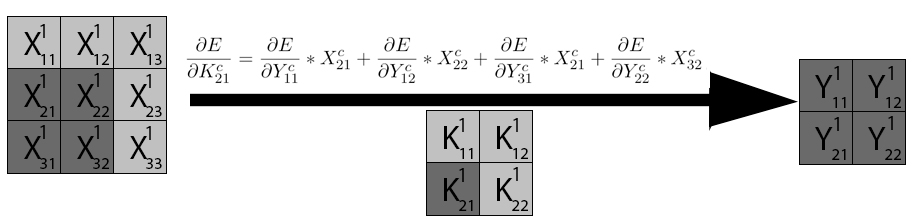
\includegraphics[width=1.4\linewidth]{imagenes/conv_backprop_3.jpg}  
		\caption{Cálculo de $\frac{\partial E}{\partial K^1_{21}}$}
	\end{subfigure}%
	\begin{subfigure}{.5\textwidth}
		\hspace{5mm}
		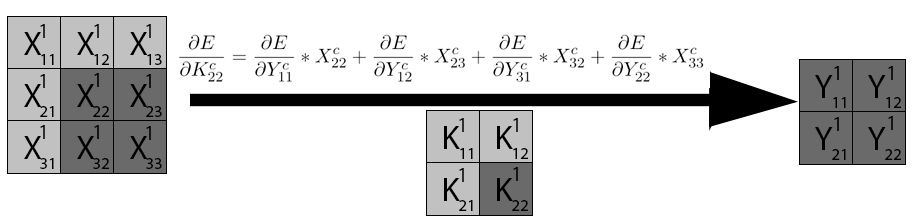
\includegraphics[width=1.4\linewidth]{imagenes/conv_backprop_4.jpg}  
		\caption{Cálculo de $\frac{\partial E}{\partial K^1_{22}}$}
	\end{subfigure}
	\caption{Cálculo del gradiente de la pérdida con respecto a cada filtro como convolución entre X e Y}
	\label{fig:conv_backprop_como_convolucion_X_Y_apendice}
\end{figure}

En la figura \ref{fig:conv_backprop_como_convolucion_X_Y_apendice}, cada subfigura $\{(a), (b), (c), (d)\}$ representa el cálculo del gradiente con respecto a un peso específico. Aunque la representación puede parecer algo diferente a simple vista, los cálculos son esencialmente los mismos que los obtenidos anteriormente, con la única diferencia en la forma en que se visualizan.

\subsection{Gradiente respecto a entrada como convolución}

Por razones de simplicidad, y en consonancia con las recomendaciones de expertos, y la experiencia personal, se empleará ReLU como función de activación en las capas convolucionales. Dado que, la derivada de esta función ya ha sido previamente calculada, (véase la fórmula \ref{deriv_relu}), se considerará esta información para los cálculos subsiguientes.


\begin{gather}
	\frac{\partial E}{\partial A^c_{11}} = \frac{\partial E}{\partial Y^c_{11}} * K^c_{11} *  ReLU'(A^c_{11}) \\
	\frac{\partial E}{\partial A^c_{12}} = (\frac{\partial E}{\partial Y^c_{11}} * K^c_{12} + \frac{\partial E}{\partial Y^c_{12}} * K^c_{11}) * ReLU'(A^c_{12}) \\
	\frac{\partial E}{\partial A^c_{13}} = \frac{\partial E}{\partial Y^c_{12}} * K^c_{12} * ReLU'(A^c_{13}) \\
\end{gather}

\begin{gather}
	\frac{\partial E}{\partial A^c_{21}} = (\frac{\partial E}{\partial Y^c_{11}} * K^c_{21} + \frac{\partial E}{\partial Y^c_{21}} * K^c_{11}) * ReLU'(A^c_{21}) \\
	\frac{\partial E}{\partial A^c_{22}} = (\frac{\partial E}{\partial Y^c_{11}} * K^c_{22} + \frac{\partial E}{\partial Y^c_{12}} * K^c_{21} + \frac{\partial E}{\partial Y^c_{21}} * K^c_{12} + \frac{\partial E}{\partial Y^c_{22}} * K^c_{11}) * ReLU'(A^c_{22}) \\
	\frac{\partial E}{\partial A^c_{23}} = (\frac{\partial E}{\partial Y^c_{12}} * K^c_{22} + \frac{\partial E}{\partial Y^c_{22}} * K^c_{12}) * ReLU'(A^c_{22})\\
\end{gather}

\begin{gather}
	\frac{\partial E}{\partial A^c_{31}} = \frac{\partial E}{\partial Y^c_{21}} * K^c_{21} * ReLU'(A^c_{31})\\
	\frac{\partial E}{\partial A^c_{32}} = (\frac{\partial E}{\partial Y^c_{21}} * K^c_{22} + \frac{\partial E}{\partial Y^c_{22}} * K^c_{21}) * ReLU'(A^c_{32})\\
	\frac{\partial E}{\partial A^c_{33}} = \frac{\partial E}{\partial Y^c_{22}} * K^c_{22} * ReLU'(A^c_{33})
\end{gather}

Tal y como se observa en los cálculos obtenidos, estos corresponden a una convolución de tipo ``full'' (completa) entre el gradiente con respecto a la capa de salida (Y) y los pesos (K), invertidos tanto horizontal como verticalmente. El proceso de cálculo del gradiente con respecto a cada valor $x \in X$ se presenta en detalle en la figura \ref{fig:conv_backprop_como_convolucion_Y_W_apendice}, mientras que la manera de invertir los pesos se ilustra en la figura \ref{fig:flip_W_apendice} \cite{conv_backprop}.

\begin{figure}[H]
	\centering
	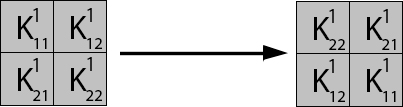
\includegraphics[width=0.8\linewidth]{imagenes/flip_pesos.jpg}  
	\caption{Inversión de los pesos en K tanto horizontal como verticalmente}
	\label{fig:flip_W_apendice}
\end{figure}

\begin{figure}[H]
	\centering
	\begin{subfigure}{.5\textwidth}
		\hspace{-25mm}
		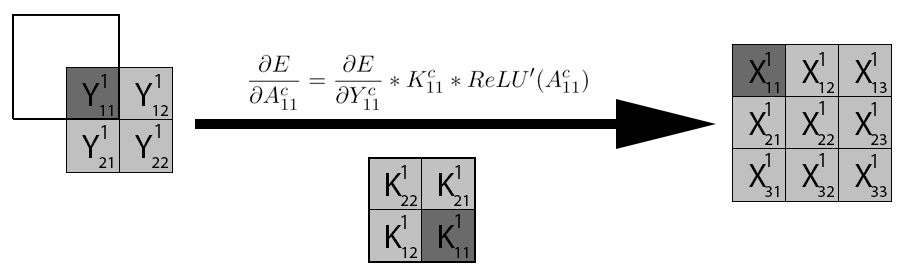
\includegraphics[width=1.4\linewidth]{imagenes/conv_back_entrada_1.jpg}  
		\caption{Gradiente con respecto a $X^1_{11}$}
	\end{subfigure}%
	\begin{subfigure}{.5\textwidth}
		\hspace{5mm}
		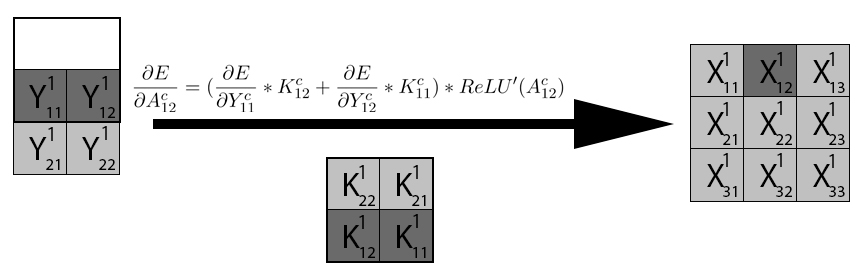
\includegraphics[width=1.4\linewidth]{imagenes/conv_back_entrada_2.jpg}  
		\caption{Gradiente con respecto a $X^1_{12}$}
	\end{subfigure}
	\vspace{5mm}
	\begin{subfigure}{.5\textwidth}
		\hspace{-25mm}
		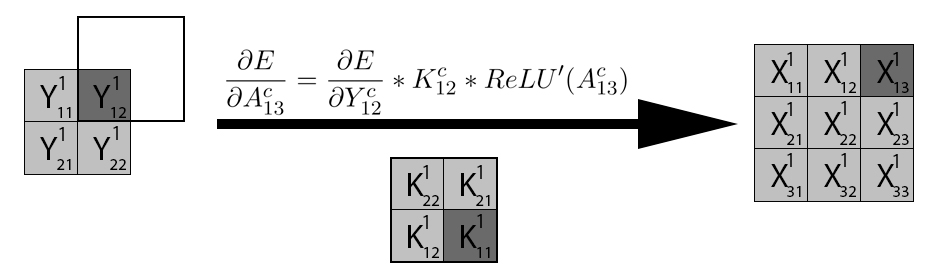
\includegraphics[width=1.4\linewidth]{imagenes/conv_back_entrada_3.jpg}  
		\caption{Gradiente con respecto a $X^1_{13}$}
	\end{subfigure}%
	\begin{subfigure}{.5\textwidth}
		\hspace{5mm}
		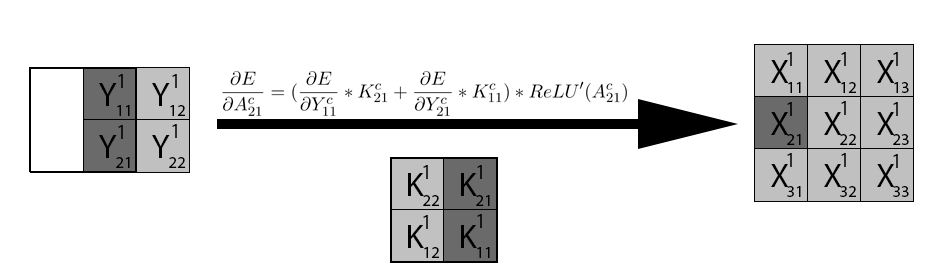
\includegraphics[width=1.4\linewidth]{imagenes/conv_back_entrada_4.jpg}  
		\caption{Gradiente con respecto a $X^1_{21}$}
	\end{subfigure}
	\vspace{5mm}
	\begin{subfigure}{.5\textwidth}
		\hspace{-25mm}
		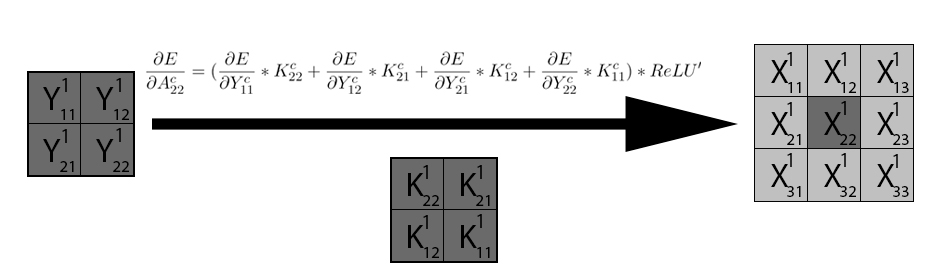
\includegraphics[width=1.4\linewidth]{imagenes/conv_back_entrada_5.jpg}  
		\caption{Gradiente con respecto a $X^1_{22}$}
	\end{subfigure}%
	\begin{subfigure}{.5\textwidth}
		\hspace{5mm}
		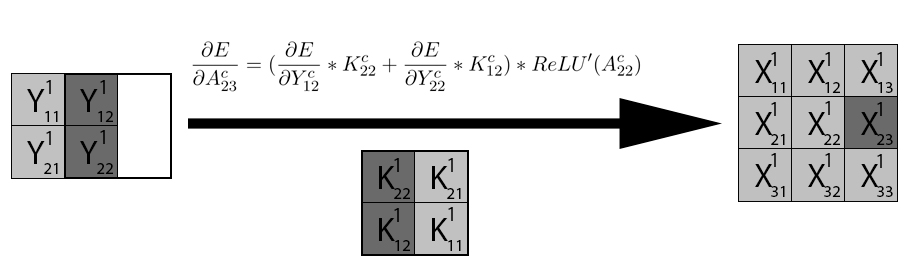
\includegraphics[width=1.4\linewidth]{imagenes/conv_back_entrada_6.jpg}  
		\caption{Gradiente con respecto a $X^1_{23}$}
	\end{subfigure}
	\vspace{5mm}
	\begin{subfigure}{.5\textwidth}
		\hspace{-25mm}
		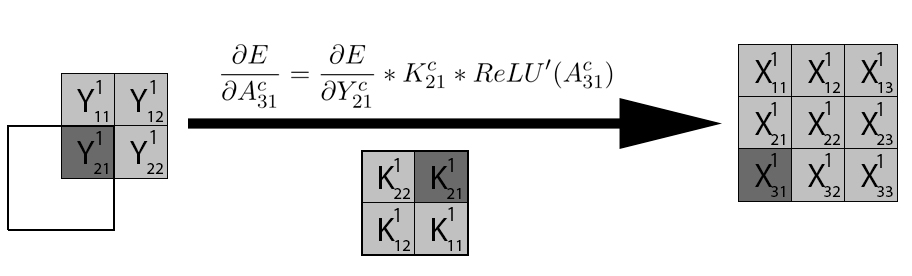
\includegraphics[width=1.4\linewidth]{imagenes/conv_back_entrada_7.jpg}  
		\caption{Gradiente con respecto a $X^1_{31}$}
	\end{subfigure}%
	\begin{subfigure}{.5\textwidth}
		\hspace{5mm}
		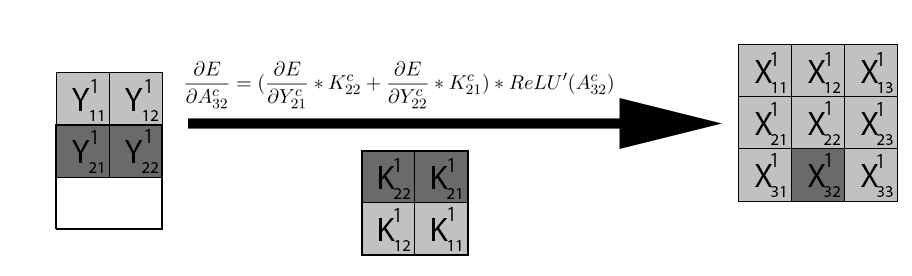
\includegraphics[width=1.4\linewidth]{imagenes/conv_back_entrada_8.jpg}  
		\caption{Gradiente con respecto a $X^1_{32}$}
	\end{subfigure}
	\vspace{5mm}
	\begin{subfigure}{.5\textwidth}
		\hspace{-25mm}
		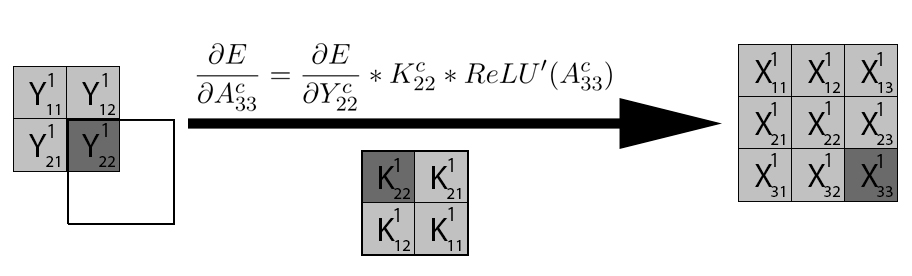
\includegraphics[width=1.4\linewidth]{imagenes/conv_back_entrada_9.jpg}  
		\caption{Gradiente con respecto a $X^1_{33}$}
	\end{subfigure}
	\caption{Cálculo del gradiente de la pérdida con respecto a cada valor de entrada como convolución entre K e Y}
	\label{fig:conv_backprop_como_convolucion_Y_W_apendice}
\end{figure}

Una vez más, los cálculos presentados en la Figura \ref{fig:conv_backprop_como_convolucion_Y_W} coinciden perfectamente con los obtenidos anteriormente, ya que son idénticos. La única diferencia radica en la manera de presentación, la cual ha sido adaptada para ofrecer una comprensión más y generalizada del proceso. Esta adaptación facilita la automatización de los cálculos y permite una implementación más eficiente en el código.

\section{Retropropagación con relleno}

\begin{figure}[H]
	\centering
	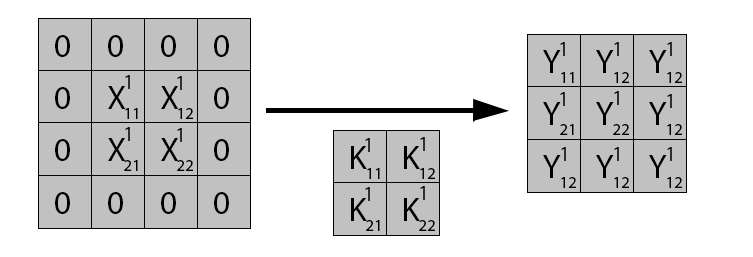
\includegraphics[width=0.8\linewidth]{imagenes/conv_back_padding_intro.jpg} 
	\caption{Ejemplo de retropropagación en una capa convolucional con relleno}
	\label{fig:conv_back_padding_intro}
\end{figure}

De manera similar al apartado anterior, se realizará y presentará el cálculo de la retropropagación para una capa convolucional. La diferencia principal en este caso radica en la inclusión de relleno en la capa, como se ilustra en el ejemplo proporcionado en la Figura \ref{fig:conv_back_padding_intro}. En consecuencia, se procederá a calcular el gradiente de la función de error con respecto a los pesos y a los valores de entrada de la capa.

\subsection{Gradiente de $Y^c_{11}$}

\begin{figure}[H]
	\centering
	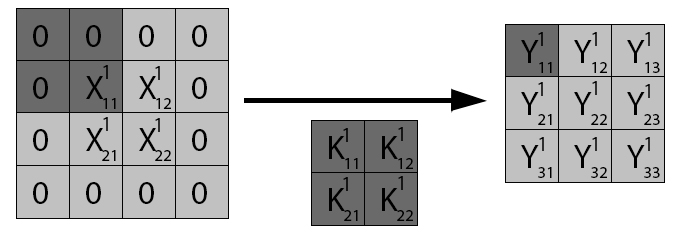
\includegraphics[width=0.8\linewidth]{imagenes/conv_back_padding_1.jpg} 
	\caption{Retropropagación de $Y^c_{11}$}
\end{figure}

Para facilitar la compresión del lector, se conservará la misma estructura y notación empleadas en el apartado anterior. Así, se procederá al cálculo del gradiente de $Y^c_{11}$ con respecto a cada peso utilizando las fórmulas \ref{gradr_Y11_w_1} y \ref{gradr_Y11_w_1}.

\begin{gather}
	Y^c_{11} = Z^c_{11} * K^c_{22} \\
	\frac{\partial Y^c_{11}}{\partial K^c_{xy}} = \frac{\partial (Z^c_{11} * K^c_{22})}{\partial K^c_{xy}} \\
	\frac{\partial Y^c_{11}}{\partial K^c_{11}} = 0, \hspace{10mm} \frac{\partial Y^c_{11}}{\partial K^c_{12}} = 0 \hspace{3mm} \label{gradr_Y11_w_1} \\
	\frac{\partial Y^c_{11}}{\partial K^c_{21}} = 0, \hspace{10mm} \frac{\partial Y^c_{11}}{\partial K^c_{22}} = Z^c_{11} \label{gradr_Y11_w_2}
\end{gather}

Para mantener la coherencia con el apartado anterior, también se calculará el gradiente de $Y^c_{11}$ con respecto a cada valor del volumen de entrada utilizando las fórmulas \ref{gradr_Y11_z_1} y \ref{gradr_Y11_z_2}.

\begin{gather}
	\frac{\partial Y^c_{11}}{\partial Z^c_{11}} = K^c_{22}, \hspace{10mm} \frac{\partial Y^c_{11}}{\partial Z^c_{12}} = 0 \label{gradr_Y11_z_1} \\
	\frac{\partial Y^c_{11}}{\partial Z^c_{21}} = 0, \hspace{14mm} \frac{\partial Y^c_{11}}{\partial Z^c_{22}} = 0 \label{gradr_Y11_z_2}
\end{gather}


\subsection{Gradiente de $Y^c_{12}$}

\begin{figure}[H]
	\centering
	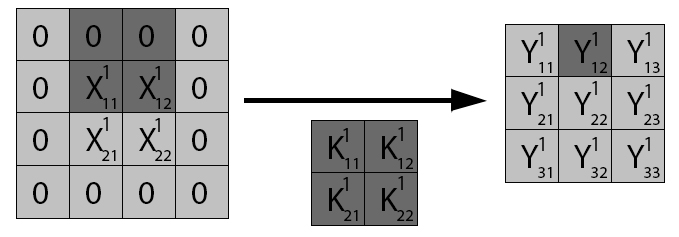
\includegraphics[width=0.8\linewidth]{imagenes/conv_back_padding_2.jpg} 
	\caption{Retropropagación de $Y^c_{12}$}
\end{figure}

Se calculará el gradiente de $Y^c_{12}$ con respecto a cada peso utilizando las fórmulas \ref{gradr_Y12_w_1} y \ref{gradr_Y12_w_2}.

\begin{gather}
	Y^c_{12} = Z^c_{11} * K^c_{21} + Z^c_{12} * K^c_{22} \\
	\frac{\partial Y^c_{12}}{\partial K^c_{xy}} = \frac{\partial (Z^c_{11} * K^c_{21} + Z^c_{12} * K^c_{22})}{\partial K^c_{xy}} \\
	\frac{\partial Y^c_{12}}{\partial K^c_{11}} = 0, \hspace{10mm} \frac{\partial Y^c_{12}}{\partial K^c_{12}} = 0 \label{gradr_Y12_w_1} \\
	\frac{\partial Y^c_{12}}{\partial K^c_{21}} = Z^c_{11}, \hspace{10mm} \frac{\partial Y^c_{12}}{\partial K^c_{22}} = Z^c_{12} \label{gradr_Y12_w_2}
\end{gather}

Asimismo, se calculará el gradiente de $Y^c_{12}$ con respecto a cada valor del volumen de entrada utilizando las fórmulas \ref{gradr_Y12_z_1} y \ref{gradr_Y12_z_2}.

\begin{gather}
	\frac{\partial Y^c_{12}}{\partial Z^c_{11}} = K^c_{21}, \hspace{10mm} \frac{\partial Y^c_{12}}{\partial Z^c_{12}} = K^c_{22} \label{gradr_Y12_z_1} \\
	\frac{\partial Y^c_{12}}{\partial Z^c_{21}} = 0, \hspace{14mm} \frac{\partial Y^c_{12}}{\partial Z^c_{22}} = 0 \hspace{4mm} \label{gradr_Y12_z_2}
\end{gather}

\subsection{Gradiente de $Y^c_{13}$}

\begin{figure}[H]
	\centering
	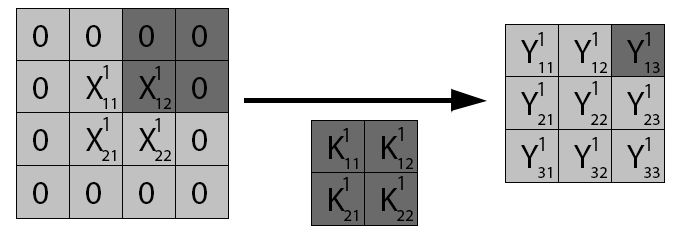
\includegraphics[width=0.8\linewidth]{imagenes/conv_back_padding_3.jpg} 
	\caption{Retropropagación de $Y^c_{13}$}
\end{figure}

Se calculará el gradiente de $Y^c_{13}$ con respecto a cada peso mediante las fórmulas \ref{gradr_Y13_w_1} y \ref{gradr_Y13_w_2}.

\begin{gather}
	Y^c_{13} = Z^c_{12} * K^c_{21} \\
	\frac{\partial Y^c_{13}}{\partial K^c_{xy}} = \frac{\partial (Z^c_{12} * K^c_{21})}{\partial K^c_{xy}} \\
	\frac{\partial Y^c_{13}}{\partial K^c_{11}} = 0, \hspace{13mm} \frac{\partial Y^c_{13}}{\partial K^c_{12}} = 0 \label{gradr_Y13_w_1} \\
	\frac{\partial Y^c_{13}}{\partial K^c_{21}} = Z^c_{12}, \hspace{10mm} \frac{\partial Y^c_{13}}{\partial K^c_{22}} = 0
\end{gather} \label{gradr_Y13_w_2}

Además, se calculará el gradiente de $Y^c_{13}$ con respecto a cada valor del volumen de entrada mediante las fórmulas \ref{gradr_Y13_z_1} y \ref{gradr_Y13_z_2}.

\begin{gather}
	\frac{\partial Y^c_{13}}{\partial Z^c_{11}} = 0, \hspace{10mm} \frac{\partial Y^c_{13}}{\partial Z^c_{12}} = K^c_{21} \label{gradr_Y13_z_1} \\
	\frac{\partial Y^c_{13}}{\partial Z^c_{21}} = 0, \hspace{14mm} \frac{\partial Y^c_{13}}{\partial Z^c_{22}} = 0 \hspace{4mm} \label{gradr_Y13_z_2}
\end{gather}


\subsection{Gradiente de $Y^c_{21}$}

\begin{figure}[H]
	\centering
	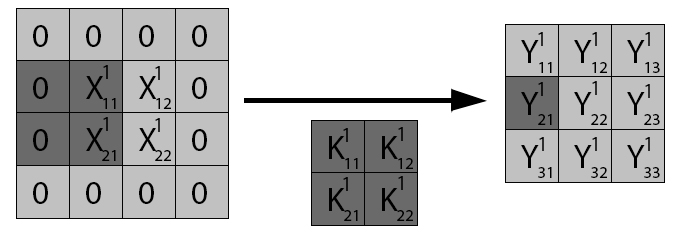
\includegraphics[width=0.8\linewidth]{imagenes/conv_back_padding_4.jpg} 
	\caption{Retropropagación de $Y^c_{21}$}
\end{figure}

Se calculará el gradiente de $Y^c_{21}$ con respecto a cada peso utilizando las fórmulas \ref{gradr_Y21_w_1} y \ref{gradr_Y21_w_2}.


\begin{gather}
	Y^c_{21} = Z^c_{11} * K^c_{12} + Z^c_{21} * K^c_{22} \\
	\frac{\partial Y^c_{21}}{\partial K^c_{xy}} = \frac{\partial (Z^c_{11} * K^c_{12} + Z^c_{21} * K^c_{22})}{\partial K^c_{xy}} \\
	\frac{\partial Y^c_{21}}{\partial K^c_{11}} = 0, \hspace{10mm} \frac{\partial Y^c_{21}}{\partial K^c_{12}} = Z^c_{11} \label{gradr_Y21_w_1} \\
	\frac{\partial Y^c_{21}}{\partial K^c_{21}} = 0, \hspace{10mm} \frac{\partial Y^c_{21}}{\partial K^c_{22}} = Z^c_{21} \label{gradr_Y21_w_2}
\end{gather}

Además, se calculará el gradiente de $Y^c_{21}$ con respecto a cada valor del volumen de entrada utilizando las fórmulas \ref{gradr_Y21_z_1} y \ref{gradr_Y21_z_2}.

\begin{gather}
	\frac{\partial Y^c_{21}}{\partial Z^c_{11}} = K^c_{12}, \hspace{10mm} \frac{\partial Y^c_{21}}{\partial Z^c_{12}} = 0 \label{gradr_Y21_z_1} \\
	\frac{\partial Y^c_{21}}{\partial Z^c_{21}} = K^c_{22}, \hspace{10mm} \frac{\partial Y^c_{21}}{\partial Z^c_{22}} = 0
\end{gather} \label{gradr_Y21_z_2}

\subsection{Gradiente de $Y^c_{22}$}

\begin{figure}[H]
	\centering
	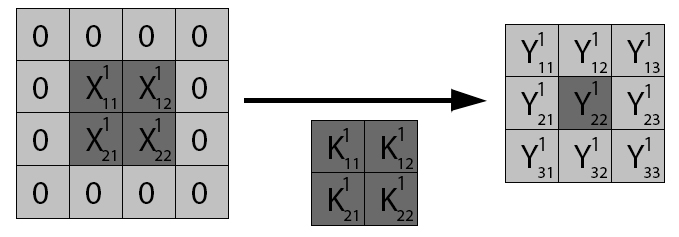
\includegraphics[width=0.8\linewidth]{imagenes/conv_back_padding_5.jpg} 
	\caption{Retropropagación de $Y^c_{22}$}
\end{figure}

Se calculará el gradiente de $Y^c_{22}$ con respecto a cada peso utilizando las fórmulas \ref{gradr_Y22_w_1} y \ref{gradr_Y22_w_2}.


\begin{gather}
	Y^c_{22} = Z^c_{11} * K^c_{11} + Z^c_{12} * K^c_{12} + Z^c_{21} * K^c_{21} + Z^c_{22} * K^c_{22} \\
	\frac{\partial Y^c_{22}}{\partial K^c_{xy}} = \frac{\partial (Z^c_{11} * K^c_{11} + Z^c_{12} * K^c_{12} + Z^c_{21} * K^c_{21} + Z^c_{22} * K^c_{22})}{\partial K^c_{xy}} \\
	\frac{\partial Y^c_{22}}{\partial K^c_{11}} = Z^c_{11}, \hspace{10mm} \frac{\partial Y^c_{22}}{\partial K^c_{12}} = Z^c_{12} \label{gradr_Y22_w_1} \\
	\frac{\partial Y^c_{22}}{\partial K^c_{21}} = Z^c_{21}, \hspace{10mm} \frac{\partial Y^c_{22}}{\partial K^c_{22}} = Z^c_{22} \label{gradr_Y22_w_2}
\end{gather}

Asimismo, se calculará el gradiente de $Y^c_{22}$ con respecto a cada valor del volumen de entrada mediante las fórmulas \ref{gradr_Y22_z_1} y \ref{gradr_Y22_z_2}.

\begin{gather}
	\frac{\partial Y^c_{22}}{\partial Z^c_{11}} = K^c_{11}, \hspace{10mm} \frac{\partial Y^c_{22}}{\partial Z^c_{12}} = K^c_{12} \label{gradr_Y22_z_1} \\
	\frac{\partial Y^c_{22}}{\partial Z^c_{21}} = K^c_{21}, \hspace{10mm} \frac{\partial Y^c_{22}}{\partial Z^c_{22}} = K^c_{22} \label{gradr_Y22_z_2}.
\end{gather}

\subsection{Gradiente de $Y^c_{23}$}

\begin{figure}[H]
	\centering
	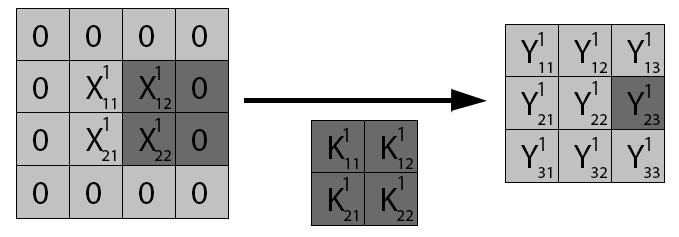
\includegraphics[width=0.8\linewidth]{imagenes/conv_back_padding_6.jpg} 
	\caption{Retropropagación de $Y^c_{23}$}
\end{figure}

Se calculará el gradiente de $Y^c_{23}$ con respecto a cada peso utilizando las fórmulas \ref{gradr_Y23_w_1} y \ref{gradr_Y23_w_2}.


\begin{gather}
	Y^c_{23} = Z^c_{12} * K^c_{11} + Z^c_{22} * K^c_{21} \\
	\frac{\partial Y^c_{23}}{\partial K^c_{xy}} = \frac{\partial (Z^c_{12} * K^c_{11} + Z^c_{22} * K^c_{21})}{\partial K^c_{xy}} \\
	\frac{\partial Y^c_{23}}{\partial K^c_{11}} = Z^c_{12}, \hspace{10mm} \frac{\partial Y^c_{23}}{\partial K^c_{12}} = 0 \label{gradr_Y23_w_1} \\
	\frac{\partial Y^c_{23}}{\partial K^c_{21}} = Z^c_{22}, \hspace{10mm} \frac{\partial Y^c_{23}}{\partial K^c_{22}} = 0 \label{gradr_Y23_w_2}
\end{gather}

De igual manera, se calculará el gradiente de $Y^c_{23}$ con respecto a cada valor del volumen de entrada mediante las fórmulas \ref{gradr_Y22_z_1} y \ref{gradr_Y22_z_2}.


\begin{gather}
	\frac{\partial Y^c_{23}}{\partial Z^c_{11}} = 0, \hspace{10mm} \frac{\partial Y^c_{23}}{\partial Z^c_{12}} = K^c_{11}\\
	\frac{\partial Y^c_{23}}{\partial Z^c_{21}} = 0, \hspace{10mm} \frac{\partial Y^c_{23}}{\partial Z^c_{22}} = K^c_{21}
\end{gather}

\subsection{Gradiente de $Y^c_{31}$}

\begin{figure}[H]
	\centering
	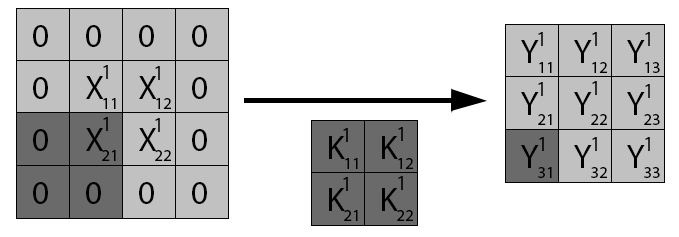
\includegraphics[width=0.8\linewidth]{imagenes/conv_back_padding_7.jpg} 
	\caption{Retropropagación de $Y^c_{31}$}
\end{figure}

Se calculará el gradiente de $Y^c_{31}$ con respecto a cada peso utilizando las fórmulas \ref{gradr_Y31_w_1} y \ref{gradr_Y31_w_2}.

\begin{gather}
	Y^c_{31} = Z^c_{21} * K^c_{12} \\
	\frac{\partial Y^c_{31}}{\partial K^c_{xy}} = \frac{\partial (Z^c_{21} * K^c_{12})}{\partial K^c_{xy}} \\
	\frac{\partial Y^c_{31}}{\partial K^c_{11}} = 0, \hspace{10mm} \frac{\partial Y^c_{31}}{\partial K^c_{12}} = Z^c_{21} \label{gradr_Y31_w_1} \\
	\frac{\partial Y^c_{31}}{\partial K^c_{21}} = 0, \hspace{10mm} \frac{\partial Y^c_{31}}{\partial K^c_{22}} = 0 \hspace{4mm} \label{gradr_Y31_w_2}
\end{gather}

Asimismo, se calculará el gradiente de $Y^c_{31}$ con respecto a cada valor del volumen de entrada mediante las fórmulas \ref{gradr_Y31_z_1} y \ref{gradr_Y31_z_2}.

\begin{gather}
	\frac{\partial Y^c_{31}}{\partial Z^c_{11}} = 0, \hspace{14mm} \frac{\partial Y^c_{31}}{\partial Z^c_{12}} = 0 \label{gradr_Y31_z_1} \\
	\frac{\partial Y^c_{31}}{\partial Z^c_{21}} = K^c_{12}, \hspace{10mm} \frac{\partial Y^c_{31}}{\partial Z^c_{22}} = 0 \label{gradr_Y31_z_2}
\end{gather}


\subsection{Gradiente de $Y^c_{32}$}

\begin{figure}[H]
	\centering
	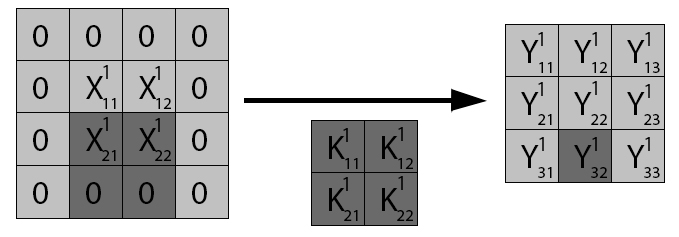
\includegraphics[width=0.8\linewidth]{imagenes/conv_back_padding_8.jpg} 
	\caption{Retropropagación de $Y^c_{32}$}
\end{figure}

Se calculará el gradiente de $Y^c_{32}$ con respecto a cada peso utilizando las fórmulas \ref{gradr_Y32_w_1} y \ref{gradr_Y32_w_2}.

\begin{gather}
	Y^c_{32} = Z^c_{21} * K^c_{11} + Z^c_{22} * K^c_{12} \\
	\frac{\partial Y^c_{32}}{\partial K^c_{xy}} = \frac{\partial (Z^c_{21} * K^c_{11} + Z^c_{22} * K^c_{12})}{\partial K^c_{xy}} \\
	\frac{\partial Y^c_{32}}{\partial K^c_{11}} = Z^c_{21}, \hspace{10mm} \frac{\partial Y^c_{32}}{\partial K^c_{12}} = Z^c_{22} \label{gradr_Y32_w_1} \\
	\frac{\partial Y^c_{32}}{\partial K^c_{21}} = 0, \hspace{14mm} \frac{\partial Y^c_{32}}{\partial K^c_{22}} = 0 \hspace{4mm} \label{gradr_Y32_w_2}
\end{gather}

Además, se calculará el gradiente de $Y^c_{32}$ con respecto a cada valor del volumen de entrada mediante las fórmulas \ref{gradr_Y32_z_1} y \ref{gradr_Y32_z_2}.


\begin{gather}
	\frac{\partial Y^c_{32}}{\partial Z^c_{11}} = 0, \hspace{14mm} \frac{\partial Y^c_{32}}{\partial Z^c_{12}} = 0 \hspace{4mm} \label{gradr_Y32_z_1} \\
	\frac{\partial Y^c_{32}}{\partial Z^c_{21}} = K^c_{11}, \hspace{10mm} \frac{\partial Y^c_{32}}{\partial Z^c_{22}} = K^c_{12} \label{gradr_Y32_z_2}
\end{gather}



\subsection{Gradiente de $Y^c_{33}$}

\begin{figure}[H]
	\centering
	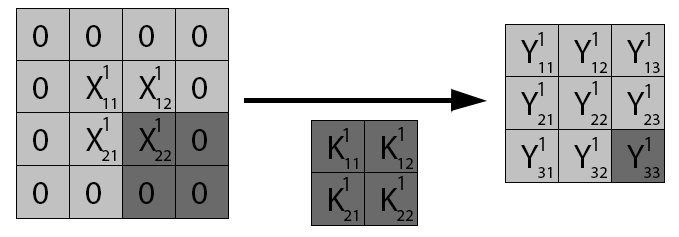
\includegraphics[width=0.8\linewidth]{imagenes/conv_back_padding_9.jpg} 
	\caption{Retropropagación de $Y^c_{33}$}
\end{figure}

Se calculará el gradiente de $Y^c_{33}$ con respecto a cada peso utilizando las fórmulas \ref{gradr_Y33_w_1} y \ref{gradr_Y33_w_2}.


\begin{gather}
	Y^c_{33} = Z^c_{22} * K^c_{11} \\
	\frac{\partial Y^c_{33}}{\partial K^c_{xy}} = \frac{\partial (Z^c_{22} * K^c_{11})}{\partial K^c_{xy}} \\
	\frac{\partial Y^c_{33}}{\partial K^c_{11}} = Z^c_{22}, \hspace{10mm} \frac{\partial Y^c_{33}}{\partial K^c_{12}} = 0 \label{gradr_Y33_w_1} \\
	\frac{\partial Y^c_{33}}{\partial K^c_{21}} = 0, \hspace{14mm} \frac{\partial Y^c_{33}}{\partial K^c_{22}} = 0 \label{gradr_Y33_w_2}
\end{gather}

Asimismo, se calculará el gradiente de $Y^c_{33}$ con respecto a cada valor del volumen de entrada utilizando las fórmulas \ref{gradr_Y33_z_1} y \ref{gradr_Y33_z_2}.


\begin{gather}
	\frac{\partial Y^c_{33}}{\partial Z^c_{11}} = 0, \hspace{10mm} \frac{\partial Y^c_{33}}{\partial Z^c_{12}} = 0 \hspace{4mm} \label{gradr_Y33_z_1} \\
	\frac{\partial Y^c_{33}}{\partial Z^c_{21}} = 0, \hspace{10mm} \frac{\partial Y^c_{33}}{\partial Z^c_{22}} = K^c_{11} \label{gradr_Y33_z_2}
\end{gather}


\subsection{Gradiente respecto a pesos como convolución}

Finalmente, de manera similar al caso anterior, se calcula la sumatoria de los gradientes y, con ello, el gradiente de la función de pérdida con respecto a cada peso $K_{xy}$. Nuevamente, se identifica un patrón claro en los resultados obtenidos.

\begin{gather}
	\frac{\partial E}{\partial K^c_{11}} = \frac{\partial E}{\partial Y^c_{22}} * Z^c_{11} + \frac{\partial E}{\partial Y^c_{23}} * Z^c_{12} + \frac{\partial E}{\partial Y^c_{32}} * Z^c_{21} + \frac{\partial E}{\partial Y^c_{33}} * Z^c_{22} \label{result_conv_1_apendice} \\
	\frac{\partial E}{\partial K^c_{12}} = \frac{\partial E}{\partial Y^c_{21}} * Z^c_{11} + \frac{\partial E}{\partial Y^c_{22}} * Z^c_{12} + \frac{\partial E}{\partial Y^c_{31}} * Z^c_{21} + \frac{\partial E}{\partial Y^c_{32}} * Z^c_{22} \label{result_conv_2_apendice} \\
	\frac{\partial E}{\partial K^c_{21}} = \frac{\partial E}{\partial Y^c_{12}} * Z^c_{11} + \frac{\partial E}{\partial Y^c_{13}} * Z^c_{12} + \frac{\partial E}{\partial Y^c_{22}} * Z^c_{21} + \frac{\partial E}{\partial Y^c_{23}} * Z^c_{22} \label{result_conv_3_apendice} \\
	\frac{\partial E}{\partial K^c_{22}} = \frac{\partial E}{\partial Y^c_{11}} * Z^c_{11} + \frac{\partial E}{\partial Y^c_{12}} * Z^c_{12} + \frac{\partial E}{\partial Y^c_{21}} * Z^c_{21} + \frac{\partial E}{\partial Y^c_{22}} * Z^c_{22} \label{result_conv_4_apendice}
\end{gather}

Como se puede observar en los cálculos obtenidos (véanse las fórmulas \ref{result_conv_1_apendice}, \ref{result_conv_2_apendice}, \ref{result_conv_3_apendice}, y \ref{result_conv_4_apendice}), estos coinciden con una convolución entre la entrada X con relleno, y el gradiente con respecto a la capa de salida Y, como se ilustra en la Figura \ref{fig:conv_backprop_como_convolucion_Xpad_Y}. Como era de esperar, los resultados son equivalentes a los obtenidos ene el caso anterior, con la única diferencia de que ahora se emplea X con relleno en lugar de X sin relleno para realizar la convolución.

\begin{figure}[H]
	\centering
	\begin{subfigure}{.5\textwidth}
		\hspace{-25mm}
		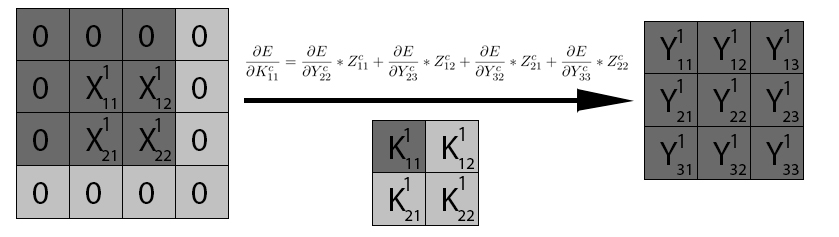
\includegraphics[width=1.4\linewidth]{imagenes/conv_back_pad_1.jpg}  
		\caption{Cálculo de $\frac{\partial E}{\partial K^1_{11}}$}
	\end{subfigure}%
	\begin{subfigure}{.5\textwidth}
		\hspace{5mm}
		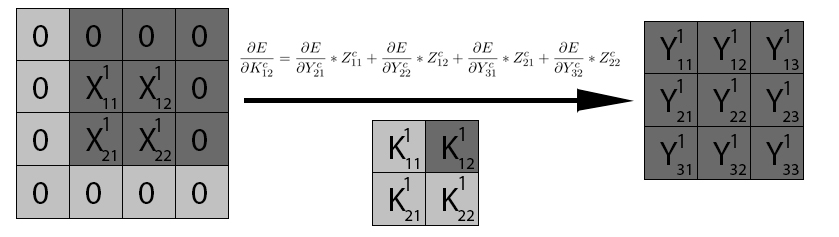
\includegraphics[width=1.4\linewidth]{imagenes/conv_back_pad_2.jpg}  
		\caption{Cálculo de $\frac{\partial E}{\partial K^1_{12}}$}
	\end{subfigure}
	\vspace{5mm}
	\begin{subfigure}{.5\textwidth}
		\hspace{-25mm}
		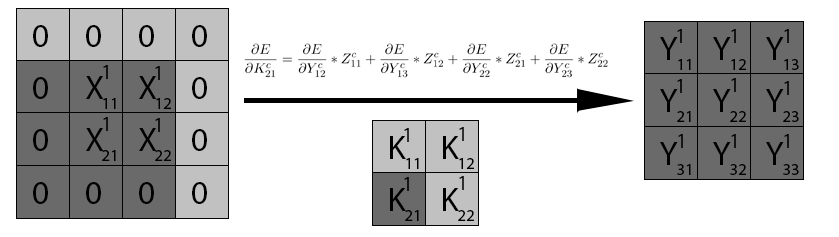
\includegraphics[width=1.4\linewidth]{imagenes/conv_back_pad_3.jpg}  
		\caption{Cálculo de $\frac{\partial E}{\partial K^1_{21}}$}
	\end{subfigure}%
	\begin{subfigure}{.5\textwidth}
		\hspace{5mm}
		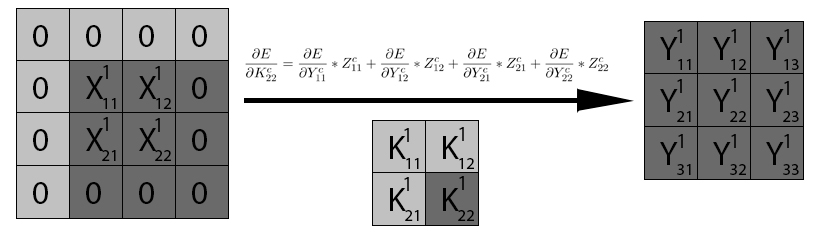
\includegraphics[width=1.4\linewidth]{imagenes/conv_back_pad_4.jpg}  
		\caption{Cálculo de $\frac{\partial E}{\partial K^1_{22}}$}
	\end{subfigure}
	\caption{Cálculo del gradiente de la pérdida con respecto a cada filtro como convolución entre X e Y}
	\label{fig:conv_backprop_como_convolucion_Xpad_Y}
\end{figure}

\subsection{Gradiente respecto a entrada como convolución}

Una vez más, se utilizará la función de activación ReLU en las capas convolucionales, conforme a lo discutido anteriormente. Por consiguiente, la derivada de esta función ya ha sido determinada previamente (véase la fórmula \ref{deriv_relu}).


\begin{gather}
	\frac{\partial E}{\partial A^c_{11}} = (\frac{\partial E}{\partial Y^c_{11}} * K^c_{22} + \frac{\partial E}{\partial Y^c_{12}} * K^c_{21} + \frac{\partial E}{\partial Y^c_{21}} * K^c_{12} + \frac{\partial E}{\partial Y^c_{22}} * K^c_{11}) *  ReLU'(A^c_{11}) \label{result_conv_x1} \\
	\frac{\partial E}{\partial A^c_{12}} = (\frac{\partial E}{\partial Y^c_{12}} * K^c_{22} + \frac{\partial E}{\partial Y^c_{13}} * K^c_{21} + \frac{\partial E}{\partial Y^c_{22}} * K^c_{12} + \frac{\partial E}{\partial Y^c_{23}} * K^c_{11}) * ReLU'(A^c_{21}) \label{result_conv_x2} \\
	\frac{\partial E}{\partial A^c_{21}} = (\frac{\partial E}{\partial Y^c_{21}} * K^c_{22} + \frac{\partial E}{\partial Y^c_{22}} * K^c_{21} + \frac{\partial E}{\partial Y^c_{31}} * K^c_{12} + \frac{\partial E}{\partial Y^c_{32}} * K^c_{11}) * ReLU'(A^c_{21}) \label{result_conv_x3} \\
	\frac{\partial E}{\partial A^c_{22}} = (\frac{\partial E}{\partial Y^c_{22}} * K^c_{22} + \frac{\partial E}{\partial Y^c_{23}} * K^c_{21} + \frac{\partial E}{\partial Y^c_{32}} * K^c_{12} + \frac{\partial E}{\partial Y^c_{33}} * K^c_{11}) * ReLU'(A^c_{22}) \label{result_conv_x4}
\end{gather}

Como se observa en los cálculos obtenidos (véanse las fórmulas \ref{result_conv_x1}, \ref{result_conv_x2}, \ref{result_conv_x3}, y \ref{result_conv_x4}), los resultados coinciden con una convolución entre el gradiente con respecto a la capa de salida Y y los pesos K, invertidos tanto horizontal como verticalmente. Este proceso se ilustra en detalle en la figura \ref{fig:conv_backprop_como_convolucion_Y_K_pad}.

\begin{figure}[H]
	\centering
	\begin{subfigure}{.5\textwidth}
		\hspace{-25mm}
		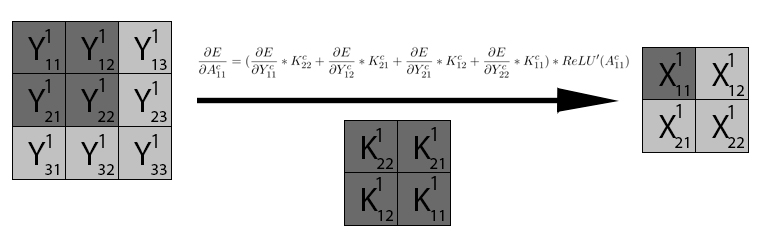
\includegraphics[width=1.4\linewidth]{imagenes/conv_back_entrada_pad_1.jpg}  
		\caption{Cálculo de $\frac{\partial E}{\partial A^1_{11}}$}
	\end{subfigure}%
	\begin{subfigure}{.5\textwidth}
		\hspace{5mm}
		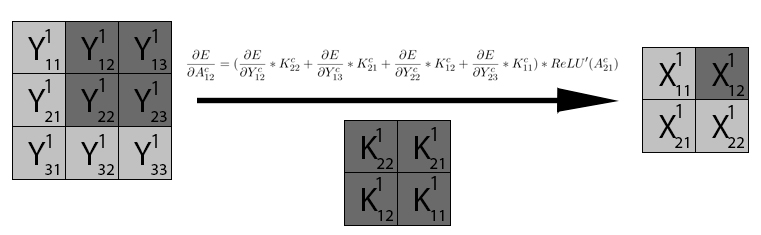
\includegraphics[width=1.4\linewidth]{imagenes/conv_back_entrada_pad_2.jpg}  
		\caption{Cálculo de $\frac{\partial E}{\partial A^1_{12}}$}
	\end{subfigure}
	\vspace{5mm}
	\begin{subfigure}{.5\textwidth}
		\hspace{-25mm}
		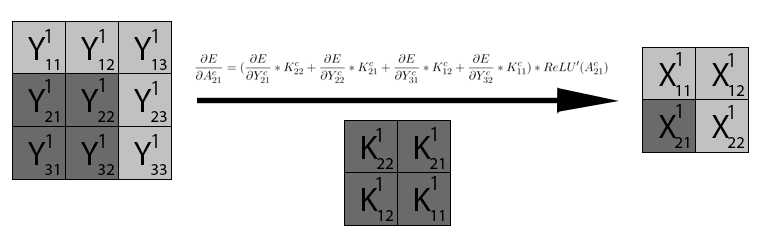
\includegraphics[width=1.4\linewidth]{imagenes/conv_back_entrada_pad_3.jpg}  
		\caption{Cálculo de $\frac{\partial E}{\partial A^1_{21}}$}
	\end{subfigure}%
	\begin{subfigure}{.5\textwidth}
		\hspace{5mm}
		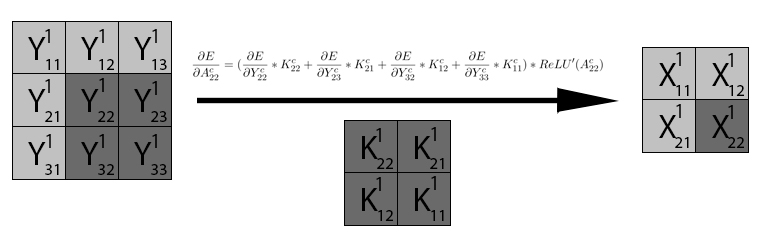
\includegraphics[width=1.4\linewidth]{imagenes/conv_back_entrada_pad_4.jpg}  
		\caption{Cálculo de $\frac{\partial E}{\partial A^1_{22}}$}
	\end{subfigure}
	\caption{Cálculo del gradiente de la pérdida con respecto a la entrada como convolución}
	\label{fig:conv_backprop_como_convolucion_Y_K_pad}
\end{figure}

Una vez desarrolladas ambas retropropagaciones en una capa convolucional, tanto con relleno como sin relleno, se pueden comparar las figuras \ref{fig:conv_backprop_como_convolucion_Y_W_apendice} y \ref{fig:conv_backprop_como_convolucion_Y_K_pad}. Em ambas representaciones, se calcula el gradiente de la pérdida con respecto al volumen de entrada. No obstante, se observa que en la primera figura se utiliza una convolución con relleno completo sobre el volumen Y (volumen de salida de la capa), mientras que en la segunda figura se aplica una convolución sin relleno.


\begin{figure}[H]
	\centering
	\begin{subfigure}{.5\textwidth}
		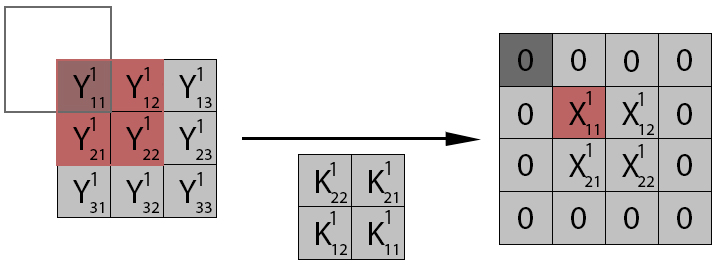
\includegraphics[width=1.4\linewidth]{imagenes/full_vs_normal_conv_1.jpg}  
		\caption{Retropropagación con un nivel de relleno}
	\end{subfigure}
	
	\vspace{5mm}
	\begin{subfigure}{.5\textwidth}
		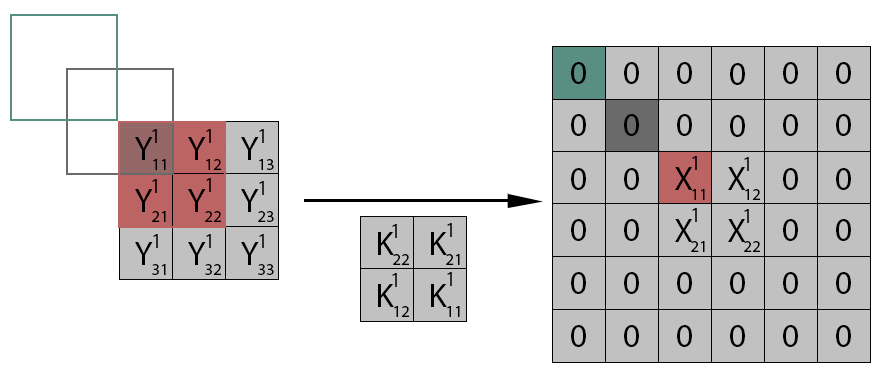
\includegraphics[width=1.4\linewidth]{imagenes/full_vs_normal_conv_2.jpg}  
		\caption{Retropropagación con dos niveles de relleno}
	\end{subfigure}
	\caption{Cálculo del gradiente de la pérdida con respecto a la entrada X con uno y dos niveles de relleno}
	\label{fig:conv_full_vs_normal_apendice}
\end{figure}

La razón detrás de esta diferencia se detalla en la figura \ref{fig:conv_full_vs_normal_apendice}. En el caso de una convolución con relleno completo, los gradientes se calculan comenzando desde la esquina superior izquierda de X. Sin embargo, dado que X incluye relleno, no es necesario calcular los gradientes en las posiciones de relleno, ya que estos valores no influyen en los cálculos posteriores.